% //////////////////// Preambolo /////////////////

% Definizione del documento
\documentclass[12pt,a4paper,oneside,hidelinks]{report}

% Lingue usate nel documento e dizionario per la correzione delle parole
\usepackage[english,italian]{babel}

%Codifica dei font di input e di output
\usepackage[T1]{fontenc}
\usepackage[utf8]{inputenc}

% Fornisce i comandi per una buona interlinea dei caratteri
\usepackage{setspace}

% Grafica del documento
\usepackage{graphicx}

% Migliore indentazione del testo
\usepackage{indentfirst}

% Gestisce le caption delle immagini
\usepackage{caption}

% Gestiscono la parte matematica del documento
\usepackage{amssymb, amsmath, amsthm}

% Gestisce il codice del documento
\usepackage{listings}

% Gestisce i link
\usepackage{hyperref}

% Formattazione pagina
\usepackage{geometry}

% Colori
\usepackage{xcolor}

% Pacchetti usati per scrivere lo pseudocodice di un algoritmo
\usepackage{algorithm}
\usepackage[noend]{algpseudocode}

%Rimuove la parola "Algorithm #" dallo pseudocodice
%\captionsetup[algorithm]{labelformat=empty}

% Gestione delle multirighe in una tabella
\usepackage{multirow}

% Gestione delle tabelle su più pagine
\usepackage{subcaption}

% Consente di impostare le virgolette del discorso diretto
\usepackage{dirtytalk}

% Allineamento dei numeri in una tabella
\usepackage{siunitx}

% Converte file eps in pdf
\usepackage{epstopdf}

% //////////////////////////////////////////////////

% Impostare interlinea a 1.5
\renewcommand{\baselinestretch}{1.5}

% Dichiara la funzione argmin non presente di default
\DeclareMathOperator*{\argmin}{argmin}

% Dichiara la funzione sgn non presente di default 
\DeclareMathOperator*{\sgn}{sgn}

% Apertura del pdf con il 100% di zoom
\hypersetup{pdfstartview={XYZ null null 1.00}}

% Impostare i margini della pagina
\geometry{left=2cm,right=2cm, top=2cm, bottom=2cm}

% Definizione della cartella contenente le immagini da usare
\graphicspath{ {img/} }

%Impostare font del documento (Latin Modern Roman)
\renewcommand*\rmdefault{lmr}

% Definizione dei colori per i commenti, le keyword e le stringhe dei codici
\definecolor{bluekeywords}{rgb}{0.13,0.13,1}
\definecolor{greencomments}{rgb}{0,0.5,0}
\definecolor{redstrings}{rgb}{0.9,0,0}

% Opzioni grafiche delle liste contenenti il codice scritto in Python
\lstdefinestyle{customp}{
    language=Python, 
    basicstyle=\ttfamily\footnotesize,   
    backgroundcolor=\color{gray!10},
    frame=none,
    tabsize=2,
    commentstyle=\color{greencomments},
    keywordstyle=\color{bluekeywords},
    stringstyle=\color{redstrings},
    title=\lstname,    
    escapeinside={\%*}{*)},
    breaklines=true,
    breakatwhitespace=true,    
    framextopmargin=2pt,
    framexbottommargin=2pt,
    inputencoding=utf8,
    extendedchars=true,
    showstringspaces=false,
    literate={à}{{\'a}}1 {ã}{{\~a}}1 {é}{{\'e}}1 {ù}{{\'u}}1,
}

% //////////////////// DOCUMENTO /////////////////

\begin{document}

% //////////////////// Titolo /////////////////

%Titolo e intestazione
\title{% 
        Predizione della funzione delle proteine \\
        con metodi di Machine Learning}
  
\author{Federico Picetti \\
        Michele Valsesia}

\date{Anno accademico 2017/2018} 

\maketitle

\tableofcontents

% //////////////////// Capitoli /////////////////

\newpage

\section*{Introduzione}
L'obiettivo del progetto consiste nel predire la funzione delle proteine del \textit{Drosophila melanogaster}, un moscerino della frutta, nonché organismo modello per gli insetti, usando i classificatori prodotti da determinati algoritmi di apprendimento. 

Per affrontare il problema, si è puntato su modelli semplici, rapidi, che consentano di ottenere una buona valutazione dell'errore di classificazione. Gli algoritmi di apprendimento scelti sono: 

\begin{itemize}
    \item Support Vector Machine (SVM)
    \item AdaBoost
\end{itemize}

Ognuno dei metodi sopra elencati verrà applicato alla predizione dei termini MF (Molecular Function) e CC (Cellular Component) della GO (Gene Ontology).

\paragraph*{}
Il progetto è stato implementato usando il linguaggio \textit{Python}, più precisamente la versione 3.5, e la versione 0.18.1 della libreria per l'apprendimento automatico \textit{scikit-learn}. Il caricamento e l'elaborazione delle strutture dati è eseguito dalla versione 0.19.1 della libreria \textit{SciPy}.

\paragraph*{}
L'elaborato descrive i passaggi e le problematiche affrontate durante lo svolgimento del lavoro. Per fare ciò, si è deciso di associare ad ogni singolo stadio lavorativo un capitolo. 

Il \autoref{chap:dati} analizza i dati di input, mostrando la loro struttura e le possibili metodologie di elaborazione. 

Il \autoref{chap:metodi} spiega i metodi di machine learning scelti e la loro implementazione pratica. 

Il \autoref{chap:risultati}, l'ultimo, illustra i risultati ottenuti dai clasificatori usando dei grafici e confronta gli algoritmi allo scopo di individuare quello che commette il più basso errore di classificazione.

\chapter{Analisi dei Dati} 
\label{chap:dati}
Le feature degli esempi da fornire in input agli algoritmi di apprendimento sono contenute in una matrice bidimensionale chiamata \textit{Matrice di Adiacenza}, mentre le rispettive etichette si trovano nella \textit{Matrice delle Annotazioni}.

Ogni ontologia è composta da un numero diverso di classi, questo significa che si hanno diverse \textit{Matrici delle Annotazioni}.

\paragraph*{}
La \textit{Matrice di Adiacenza} è una matrice quadrata simmetrica ed ha una dimensione effettiva di $3195 \times 3195$. Ogni riga identifica una proteina mentre le rispettive colonne rappresentano le feature della proteina stessa. Le entry della matrice contengono una misura di similarità, ricavata da fattori biologici, fra coppie di proteine.
Ciascuna entry può assumere valori tra $[0,1]$. Un valore vicino o uguale a 0 indica che le proteine non sono simili tra loro, mentre valori tendenti o uguali a 1 ne sanciscono la similarità. 
La matrice risulta essere sparsa, a causa dell'elevato numero di entry pari a 0.

\paragraph*{}
La \textit{Matrice delle Annotazioni} è una matrice rettangolare con un numero di righe pari al numero delle proteine e tante colonne quante sono le classi dell'ontologia considerata.

Il numero delle classi per ciascuna ontologia è descritto di seguito:

\begin{itemize}
    \item Cellular Component (CC) si compone di 235 classi
    \item Molecular Function (MF) si compone di 234 classi
\end{itemize}
  
Per ridurre lo spazio in memoria centrale e garantire una rapida elaborazione dei dati, la Matrice delle Adiacenze e la Matrice delle Annotazioni vengono entrambe caricate e convertite in matrici sparse. La funzione utilizzata per la conversione è contenuta nella libreria SciPy.

Le singole colonne delle matrici delle Annotazioni verranno successivamente convertite in array densi, in modo da poterle passare in input ai diversi algoritmi di apprendimento. 

Le classi delle Matrici delle Annotazioni vengono trattate come se fossero indipendenti tra loro, non tenendo conto della gerarchia presente. I classificatori scelti verranno addestrati sulle singole classi e le loro prestazioni saranno valutate a partire dai risultati prodotti. Verrà anche analizzato il loro comportamento al variare della classe considerata.

\chapter{Metodi di Machine Learning} 
\label{chap:metodi}

I metodi di Machine Learning scelti si basano su modelli semplici, rapidi, che consentono di ottenere una buona valutazione dell'errore di classificazione. Gli algoritmi di apprendimento considerati sono le \textit{Support Vector Machine (SVM)} e \textit{AdaBoost}. La scelta dei metodi è stata effettuata con lo scopo di individuare le differenze tra i modelli di classificazione per decretare quello che funziona meglio. Un'ulteriore motivo è dato dal voler confrontare algoritmi di apprendimento lineari, come SVM, con algoritmi basati sull'utilizzo di un numero maggiore di classificatori, come AdaBoost.

\paragraph*{}
Per poter effettuare il tuning degli iperparametri, sono state create diverse configuarazioni di esecuzione.
Le configurazioni sono inserite in un dizionario Python che ha come chiavi i nomi delle configurazioni stesse e come oggetti i classificatori della liberia scikit-learn con impostati i parametri che si vogliono testare.
Utilizzando tutte le classi di un ontologia, si ottiene un elevato tempo computazionale per ciascuna configurazione. Per evitare ciò, si è deciso di campionare le classi, prendendone una ogni cinque.
 

\section{Support Vector Machine}
Una \textit{Support Vector Machine}, comunemente abbreviata in \textit{SVM}, costruisce un iperpiano, o una serie di iperpiani, in uno spazio iperdimensionale, in modo da poter risolvere problemi di classificazione e di regressione. Una buona separazione dei dati si verifica quando si ottiene un iperpiano che massimizza la distanza dal più vicino esempio di ogni classe, in altro modo, quando si individua l'iperpiano di margine massimo. In generale, più è ampio il margine, più l'errore di classificazione sarà basso.

SVM ricava l'iperpiano di margine massimo risolvendo il seguente problema di ottimizzazione lineare convessa

\begin{equation} \label{uno}
\begin{split}
\min_ {w, b, \zeta} \frac{1}{2} w^T w + C \sum_{i=1}^{n} \zeta_i \\
\textrm {subject to } & y_i (w^T \phi (x_i) + b) \geq 1 - \zeta_i, \\
& \zeta_i \geq 0, i=1, \dotsc ,n
\end{split}
\end{equation}

La sua funzione di decisione è definita come:

\begin{equation} \label{due}
\sgn(\sum_{i=1}^n y_i \alpha_i K(x_i, x) + \rho)
\end{equation}

I support vectors sono gli esempi del training set che, a seconda dell'iperpiano ottenuto, hanno un margine inferiore o pari a 1. La soluzione prodotta da SVM dipende solo da questi esempi.

\paragraph*{}
L'apprendimento del classificatore è stato effettuato usando la funzione \textit{SVC} \footnote{\url{scikit-learn.org/stable/modules/generated/sklearn.svm.SVC.html}}, implementata nel modulo \textit{sklearn.svm} contenente gli algoritmi SVM della libreria scikit-learn. Nella definizione del metodo sono stati impostati i seguenti parametri:

\paragraph*{}
\textbf{\textit{C}}. Penalità sull'errore commesso. È un parametro di tradeoff, un valore elevato di C crea un modello complesso che mira a classificare nel miglior modo possibile gli esempi del training set, mentre un valore piccolo comporta un modello con una funzione di decisione più semplice. È un valore di tipo float. 

\paragraph*{}
\textbf{\textit{Kernel}}. Specifica il kernel che deve essere usato dall'algoritmo. I kernel scelti per lo svolgimento del progetto sono stati:

\begin{itemize}
    \item Radial Basis Function (RBF) 
    \item Polinomiale
\end{itemize}

\paragraph*{}
\textbf{\textit{degree}}. Grado del polinomio usato dal Kernel Polinomiale. È un valore intero.

\paragraph*{}
\textbf{\textit{gamma}}. Inverso del raggio di influenza. Questo parametro stabilisce quali sono gli esempi scelti dal modello come support vectors. SVM è molto sensibile a questo parametro. Con un gamma molto grande, il raggio di influenza risulterà piccolo ed il modello sceglierà come support vectors gli elementi più vicini al margine e quelli che violano il vincolo, al contrario, un gamma piccolo comporta un raggio di influenza grande ed ogni esempio del training set sarà un support vector. È un valore di tipo float.

Un valore grande di gamma può portare a overfitting, mentre uno troppo piccolo rischia di produrre un classificatore che non riesce a discriminare al meglio le classi.

\paragraph*{}
\textbf{\textit{class\_weight}}. Parametro utilizzato per il bilanciamento di classi sbilanciate. Se non viene fornito in input, tutte le classi hanno peso unitario. Il peso di ciascuna classe può essere tarato, a seconda del risultato che si vuole ottenere, privilegiando una classe rispetto ad un'altra, oppure calcolato in maniera autonoma dalla funzione per mezzo della modalità \say{balanced}. 
Questa modalità sfrutta i valori delle etichette di una classe per aggiustare i pesi in maniera tale che risultino inversamente proporzionali alle frequenze delle classi di input. In pratica, una classe con una cardinalità molto bassa, avrà un peso alto, al contrario, una classe con cardinalità elevata avrà un peso più basso. La regola di assegnamento dei pesi è la seguente.

\begin{center}
numero\_campioni / (numero\_classi * array\_contenente\_cardinalità\_classi)
\end{center}


\subsection{Parametri}
Per determinare con quali parametri, sul dataset considerato, la SVM produce dei buoni risultati, vengono eseguite le seguenti configurazioni:

\paragraph*{}
\textbf{\textit{Unbalanced}}. Il kernel di questa configurazione è RBF. La funzione SVC viene eseguita con i parametri di default, C unitario e gamma variabile, per verificare, dall'analisi dei risultati ottenuti, la necessità di modificare gli iperparametri.

\paragraph*{}
\textbf{\textit{C crescente}}. Il kernel usato dalla configurazione è RBF. Il valore di class\_weight è \say{balanced}. Mantenendo costanti tutti gli altri parametri, C viene fatto crescere nell'intervallo $[1,3]$ in maniera discreta. Si vuole verificare che aumentando C in maniera gradata, i risultati subiscano un miglioramento.

\paragraph*{}
\textbf{\textit{C e gamma crescenti}}. Questa configurazione è identica a quella precedente, con la sola differenza di far crescere anche il parametro gamma insieme a C. I valori di entrambi vengono estratti dall'intervallo $[10^{-3}, 10^3]$ in scala logaritmica.

\paragraph*{}
\textbf{\textit{Poly}}. Viene usato un kernel polinomiale di grado 4. Il valore di class\_weight è \say{balanced}. Tutti i restanti parametri non sono stati modificati. La scelta del grado del polinomio è stata effettuata tenendo in considerazione la potenza computazionale delle macchine a disposizione.

\begin{table}[ht]%	
\centering
\caption{Configurazioni di SVM}\label{tab:b1}
\begin{tabular}{|c|c|c|S[table-parse-only = true]|S[table-parse-only = true]|c|}
\hline
Nome                    & Bilanciamento & Kernel & C        & Gamma & Degree    \\ 
\hline 
SVM\_Unbalanced         & -             & RBF    & 1.0      & auto    & -       \\
\hline 
SVM\_Balanced           & balanced      & RBF    & 1.0      & auto    & -       \\
\hline 
SVM\_Balaman            & 0:0.01 1:0.99 & RBF    & 1.0      & auto    & -       \\
\hline 
SVM\_Balanced\_C2       & balanced      & RBF    & 2.0      & auto    & -       \\
\hline 
SVM\_Balanced\_C3       & balanced      & RBF    & 3.0      & auto    & -       \\
\hline 
SVM\_Balanced\_C5       & balanced      & RBF    & 5.0      & auto    & -       \\
\hline 
SVM\_Balanced\_C7       & balanced      & RBF    & 7.0      & auto    & -       \\
\hline 
SVM\_Balanced\_C0\_G0   & balanced      & RBF    & 0.01     & 1.0e-09 & -       \\
\hline 
SVM\_Balanced\_C2\_G2   & balanced      & RBF    & 0.1      & 1.0e-08 & -       \\
\hline 
SVM\_Balanced\_C7\_G7   & balanced      & RBF    & 1.0e+05  & 0.01    & -       \\
\hline 
SVM\_Balanced\_C12\_G12 & balanced      & RBF    & 1.0e+10  & 1000.0  & -       \\
\hline 
SVM\_Balanced\_Poly\_4  & balanced      & Poly   & 1.0      & auto    & 4       \\
\hline 
\end{tabular} 
\end{table}

\paragraph*{}
La complessità in tempo di ciascuna configurazione è un $\mathcal{O}(N^2)$ rispetto al numero degli esempi del training set. La velocità di computazione diminuisce considerevolmente all'aumentare della grandezza dei parametri usati.

\section{AdaBoost}
AdaBoost (adaptive boosting) è un algoritmo incrementale che costruisce una serie di classificatori $ h_{i}:\mathbb{R}^{d}\rightarrow \{-1,+1\} $ appartenenti ad una famiglia $ \mathcal{H} $. 
Il procedimento prevede di addestrare un classificatore di base sul training set, calcolarne l'errore, creare copie del classificatore e addestrarle sullo stesso training set, bilanciando i pesi degli elementi del training set classificati scorrettamente dai classificatori precedenti. I classificatori successivi tenderanno quindi a concentrarsi sui casi più difficili.
Al termine avremo un classificatore nella forma
\[\hat{y}=\sgn(\sum_{i=1}^{T} w_{i}h_{i}(\vec{x}))\]
dove $ \vec{w} $ è un vettore di coefficienti reali (pesi) e $ T $ è il numero di classificatori.

Tipicamente per contenere i costi computazionali si sceglie una famiglia $ \mathcal{H} $ di classificatori di base molto semplici. $ T $ può essere un numero fissato o può crescere durante l'apprendimento e fermarsi secondo un dato criterio di stop.

In questo lavoro si è usata l'implementazione \texttt{sklearn.ensemble.AdaBoostClassifier}
\footnote{\url{scikit-learn.org/stable/modules/generated/sklearn.ensemble.AdaBoostClassifier.html}}.
Tra i parametri di interesse, osserviamo:

\begin{description}
\item[\texttt{base\_estimator}:]la famiglia $ \mathcal{H} $ di \emph{weak learner};
\item[\texttt{n\_estimators}:]la quantità massima di stimatori da costruire, limite oltre il quale il boosting è terminato.
In caso di aderenza perfetta, la procedura di boosting è arrestata prima del raggiungimento del limite.
\item[\texttt{learning\_rate}:] permette di ridurre il contributo di ogni classificatore.

\end{description}
 
\subsection{Parametri}
In questo lavoro sono state esplorate diverse configurazioni del predittore AdaBoost.
Come classificatore di base si è optato per un \emph{decision stump}, cioè un predittore ad albero molto semplice, che presenta un solo test, quindi una sola ramificazione e al massimo due foglie. Si è utilizzata l'implementazione dell'albero di decisione di scikit-learn\footnote{\url{scikit-learn.org/stable/modules/generated/sklearn.tree.DecisionTreeClassifier.html}}, impostandone il parametro \texttt{max\_depth} a 1.

Si è mantenuto il \texttt{learning\_rate} a 1. 

Si è variato \texttt{n\_estimators} ponendolo a 10, 50 e 100 stimatori di base.

Si sono poi modificate delle proprietà dello stimatore ad albero di base, impostando un bilanciamento del peso delle classi inversamente proporzionale alla loro frequenza, usando l'impostazione \texttt{class\_weight = \say{balanced}}, in analogia col predittore SVM.

Infine, si è tentato l'utilizzo di alberi leggermente più complessi, impostandone la \texttt{max\_depth} a 3. Questo consente di creare alberi a tre livelli di test. Normalmente alzare questo livello in un albero decisione può portare ad avvicinarsi velocemente verso l'overfitting.

La \autoref{tab:b2} elenca le impostazioni di Adaboost che si sono provate in questo lavoro.

\begin{table}[ht]%	
\centering
\caption{Configurazioni di AdaBoost}\label{tab:b2}
\begin{tabular}{|c|c|c|c|}
\hline
nome & \texttt{n\_estimators} & bilanciamento & \texttt{max\_depth} \\ 
\hline 
AdaBoost\_n10 & 10 & No & 1 \\ 
\hline 
AdaBoostDefault & 50 & No & 1 \\ 
\hline 
AdaBoost\_n100 & 100 & No & 1 \\ 
\hline 
AdaBoost\_n5\_Bal & 5 & Auto & 1 \\ 
\hline 
AdaBoost\_n10\_Bal & 10 & Auto & 1 \\ 
\hline 
AdaBoost\_n50\_Bal & 50 & Auto & 1 \\ 
\hline 
AdaBoost\_n50\_Bal\_Dep3 & 5 & Auto &  3\\ 
\hline 
\end{tabular} 
\end{table}


\section{Costruzione del software}
Il programma Python è costruito in modo tale da calcolare le funzioni di predizione per un'unica ontologia. Questa scelta è stata effettuta per facilitare la gestione del codice e dei risultati prodotti. Se si vogliono eseguire diverse ontologie bisogna mandare nuovamente in esecuzione il processo specificando l'ontologia che si vuole computare.
Tuttavia, per una singola istanza del programma, possono essere inserite più configurazioni contemporaneamente.

Gli step seguiti dall'algoritmo sono i seguenti:

\begin{itemize}
    \item Verificare che l'ontologia e le configurazioni inserite siano corrette
    \item Se ritenute valide, le configurazioni vengono eseguite una alla volta sulle classi dell'ontologia
    \item Calcolo delle metriche e salvataggio dei risultati ottenuti
\end{itemize}

\paragraph*{}
Le performance di un metodo vengono valutate con la tecnica sperimentale della 5-fold cross-validation. Questa tecnica suddivide il dataset in 5 fold, quattro dei quali vengono usati per addestrare il classificatore e il fold restante per ottenere le metriche richieste. Ogni fold deve essere utilizzato almeno una volta come test set, questo implica che per ogni classe vengono prodotti cinque classificatori, ciascuno con le proprie metriche.

I risultati ottenuti dall'esecuzione di una configurazione sono salvati in un file \textit{json} che presenta la seguente struttura:

\begin{itemize}
    \item Header
    \item Metriche dei fold di ogni classe
    \item Footer
\end{itemize}
L'\textit{Header} è un dizionario contenente le seguenti informazioni:
\begin{itemize}
    \item L'ontologia in uso
    \item L'algoritmo di apprendimento eseguito
    \item I parametri del metodo
    \item Il tempo di inizio della configurazione in formato data e ora
\end{itemize}
Le \textit{Metriche} ricavate da ciascun fold di ogni classe sono le seguenti:
\begin{itemize}
    \item Identificativo della classe (indice colonna della Matrice delle Annotazioni)
    \item Numero di esempi positivi nel fold
    \item Precision
    \item Recall
    \item F-score
    \item False Positive rate
    \item True Positive rate
    \item Auroc
    \item Auprc
\end{itemize}
Anche la struttura sopra descritta è contenuta all'interno di un dizionario. Ad ogni classe sono associati tanti dizionari quanti sono i fold.

Il \textit{Footer} è costituito da un dizionario di un solo elemento: il tempo di fine della configurazione in formato data e ora.

Dai file json prodotti vengono estratte le informazioni necessarie per la valutazione dei classificatori.

\paragraph*{}
Per poter eseguire la cross-validation e calcolare le misure richieste, vengono utilizzate delle funzioni messe a disposizione dalla libreria scikit-learn.
La funzione \textit{cross\_val\_score} è stata scelta perché consente di ridurre il tempo di computazione, assegnando l'esecuzione dei differenti fold di una classe alle diverse unità di elaborazione presenti sulla macchina.

Le metriche di un fold vengono calcolate fornendo in input alle funzioni le etichette degli esempi del test set e le predizioni computate dal classificatore. Di seguito una breve lista delle procedure utilizzate:

\begin{itemize}
\item \textit{precision\_recall\_fscore\_support} calcola la precision, la recall e la f-score di un classificatore

\item \textit{precision\_recall\_curve} computa la precision-recall-curve

\item \textit{average\_precision\_score} restituisce l'AUPRC del classificatore 

\item \textit{roc\_curve} determina la ROC

\item \textit{auc} restituisce l'AUROC del classificatore
\end{itemize}


\chapter{Analisi dei Risultati}
\label{chap:risultati}

\section{Scelta delle metriche}
Le metriche sono state scelte considerando diversi aspetti del dataset.
A causa della presenza di classi sbilanciate, che presentano un numero elevato di esempi negativi rispetto a quelli positivi, l'accuratezza non rappresenta una metrica significativa per il modello che si sta valutando.

\paragraph*{}
L'accuratezza corrisponde alla frazione delle predizioni corrette ed è definita come:

\begin{equation}
\texttt{accuracy}(y, \hat{y}) = \frac{1}{n_\text{samples}} \sum_{i=0}^{n_\text{samples}-1} 1(\hat{y}_i = y_i)
\end{equation}

Nella formula soprastante $1(x)$ è la funzione indicatrice. Come si può notare, l'accuratezza non fornisce un buon valore in caso di sbilanciamento, in quanto non è in grado di discriminare i valori positivi da quelli negativi.

\paragraph*{}
Le metriche considerate durante lo svolgimento del progetto sono la precision, la recall, la f-score, l'AUPRC e l'AUROC.

La \textit{precision} corrisponde all'abilità del classificatore di non etichettare un esempio negativo come positivo. È definita nell'intervallo $[0,1]$. Più la precision è alta, più un classificatore non scambierà gli esempi negativi per positivi.

\begin{equation}
\text{precision} = \frac{\text{TP}}{\text{TP} + \text{FP}}
\end{equation}

\paragraph*{}
La \textit{recall} rappresenta l'abilità di un classificatore di individuare gli esempi postivi. È definita nell'intervallo $[0,1]$. Più la recall è alta, più un classificatore individuerà meglio gli esempi positivi.

\begin{equation}
\text{recall} = \frac{\text{TP}}{\text{TP} + \text{FN}}
\end{equation}

\paragraph*{}
La \textit{F-score} è data dalla media armonica della precision e della recall. È definita nell'intervallo $[0,1]$. Più la f-score è alta, più un classificatore produrrà buoni risultati.

\begin{equation}
\text{F-score} = \frac{2 \times \text{precision} \times \text{recall}}{\text{precision} + \text{recall}}
\end{equation}

\paragraph*{}
L'\textit{Area Under the Precision-Recall Curve (AUPRC)} rappresenta l'area sotto la curva del grafico precision-recall. Assume valori definiti nell'intervallo $[0,1]$. Più il valore è alto, più un classificatore produrrà buoni risultati.

\paragraph*{}
L'\textit{Area Under the Receiver Operating Characteristic (AUROC)} rappresenta la probabilità che un classificatore associ un valore più alto ad un esempio positivo, scelto casualmente, rispetto ad uno negativo, sempre scelto in maniera casuale. Assume valori definiti nell'intervallo $[0,1]$. Più il valore è alto, più un classificatore produrrà buoni risultati.

\paragraph*{}
Come spiegato precedentemente, le metriche vengono calcolate per ogni fold di una classe e i risultati prodotti vengono salvati in un file json. Per poter valutare le performance di un classificatore su una classe specifica, viene fatta la media delle metriche di ciascun fold della classe.

\section{Risultati}

\subsection{Ill-defined}
Durante la fase di validazione è emerso che parte dei classificatori addestrati non ha predetto alcun esempio del test set, dando solo risposte negative. Poichè i 5 fold sono stati costruiti in modo da possedere sempre almeno un esempio positivo, questo significa che il classificatore ha commesso un errore.

Tale errore va oltre alla logica dei normali errori che può commettere un classificatore. Non avendo predetto neanche un positivo (vero o falso che sia), non si può escludere che il classificatore abbia semplicemente appreso a rispondere negativamente a qualunque input, rendendosi di fatto inutilizzabile.

Inoltre, poichè il numero di positivi è zero, il calcolo della precision è impossibile, dal momento che avremmo una divisione per zero. Di conseguenza anche F-score non è computabile. Durante il calcolo delle metriche, scikit-learn intercetta l'errore, solleva un warning e fissa precision e F-score a zero. 

Durante l'analisi delle metriche possiamo selezionare questi predittori intrinsecamente difettosi cercando tra i predittori quelli che abbiano Precision e F-score uguali a zero. Possiamo dunque misurare l'impatto di questi predittori (che denominiamo \emph{ill-defined}) e quantificarli.

Il numero di predittori \emph{ill-defined} aumenta quando il training set è sbilanciato, cioè quando si apprende da una classe che contiene poche proteine. Ovviamente anche la qualità dell'algoritmo di apprendimento è influente. Gli algoritmi che non bilanciano le classi e che non sono in grado di apprendere da pochi esempi genereranno predittori difettosi.

%grafico che mostra come varia qualche metrica e/o il numero di ill defined in base alla popolazione della classe
Il sistema 5-fold prevede che per ogni classe dell'ontologia vengano generati 5 predittori. I predittori \emph{ill-defined} possono essere numerosi, ma fintantochè una classe possiede almeno un predittore non \emph{ill-defined} possiamo concludere che sia possibile costruire un predittore funzionante.

Possiamo considerare il numero di predittori \emph{ill-defined} alla stregua di un indicatore di qualità dell'algoritmo di apprendimento. A parità di popolazione della classe, avere meno \emph{ill-defined} significa aver sfruttato meglio il valore degli esempi positivi.

I grafici della Figura~\ref{fig:ill1} e ~\ref{figure:ill12} mostrano la quantità di ill-defined di AdaBoost e di Svm tra i 5-fold dell'ontologia CC, le Figure~\ref{fig:ill13} e ~\ref{figure:ill14}, le quantità per l'ontologia MF.

Osserviamo quindi che per Adaboost la quantità di \emph{ill-defined} non presenta variazioni significative, e il valore mediano resta compreso tra 2 e 3 per i parametri analizzati.

Per SVM c'è molta meno continuità: il valore si abbassa per valori di C elevati, che però vedremo avere Precision molto bassa.

Menzione d'onore merita l'impostazione \say{SVM\_C12\_G12}, che ha prodotto solo classificatori \emph{ill-defined} per tutte le classi di entrambe le ontologie.

I classificatori difettosi sono inutilizzabili ma facili da identificare ed escludere. In un contesto applicativo reale verrebero esclusi dall'utilizzo. Pertanto le analisi che seguono filtrano il bias introdotto dai classificatori \emph{ill-defined} e analizzano sono i classificatori costruiti correttamente.

\subsection{Analisi a Livelli}
Per identificare i migliori classificatori e poterli confrontare tra loro, è stata creata una struttura a tre livelli. Nei primi due livelli, i classificatori di modelli diversi non interagiscono tra loro. In ogni livello, le ontologie sono sempre analizzate in maniera indipendente. 

Al \textit{Livello 1} vengono confrontate le metriche prodotte dalle diverse configurazioni di uno stesso classificatore. Questo metodo consente di determinare qual è il migliore classificatore per ogni famiglia di modelli. La Figura~\ref{figure:liv1.1} e la Figura~\ref{figure:liv1.2} mostrano i migliori classificatori dell'ontologia CC, mentre la Figura~\ref{figure:liv1.3} e la Figura~\ref{figure:liv1.4} quelli dell'ontologia MF.

\paragraph*{}
Il \textit{Livello 2} confronta la configurazione del classificatore che ha ottenuto i risultati migliori al livello precedente su diverse classi. Lo scopo di questa analisi consiste nel capire come un classificatore varia le sue predizioni a seconda della classe scelta. Le classi considerate sono tre e sono disposte in ordine crescente rispetto al numero di esempi positivi. L'id della classe si ottiene unendo il nome dell'ontologia usata e la relativa colonna della Matrice delle Annotazioni.
Per ciascun confronto vengono usate come metriche la precision, la recall, e la f-score.
La Figura~\ref{fig:liv2} mostra le configurazioni di AdaBoost e SVM per l'ontologia CC, mentre la Figura~\ref{figure:liv21} le configurazioni per l'ontologia MF.

\paragraph*{}
Il \textit{Livello 3} mette in relazione tra loro le migliori configurazioni dei classificatori di ogni famiglia di modelli. Le metriche considerate sono AUROC, AUPRC e f-score. La Figura~\ref{fig:liv3} mostra il confronto tra AdaBoost e SVM per l'ontologia CC, mentre la Figura~\ref{figure:liv31} quello per l'ontologia MF.

\subsection{Conclusioni}
Dall'analisi dei grafici di livello 1 di AdaBoost non emergono variazioni significative di performance attraverso i vari parametri. Ci sono diverse possibili cause:

\begin{itemize}
\item AdaBoost è in grado di risolvere i problemi di bilanciamento dopo ben poche iterazioni: imporre il bilanciamento all'albero sottostante non ha grande effetto
\item AdaBoost ferma l'iterazione dopo aver creato un numero sufficiente di alberi, anche se tale numero è inferiore al parametro impostato. Aumentare il numero di classificatori di base non migliora le prestazioni.
\end{itemize}

Si è optato per \say{AdaBoost\_n100} perchè presenta una Recall leggermente migliore rispetto alla concorrenza. Si è deciso di premiare una Recall alta perchè significa maggior capacità di adattarsi allo sbilanciamento del dominio di applicazione e perchè consente di utilizzare il classificatore come filtro per un eventuale classificatore successivo, più bilanciato e preciso.

SVM, invece, presenta una grande varianza di performance. Si è reso necessario un lavoro di esplorazione prima di trovare un classificatore accettabile, che non presenti Precision o Recall eccessivamente basse. \say{SVM\_Balanced\_C7\_G7} è una scelta quasi obbligata.

% //////////////////// ILL-DEFINED /////////////////

\topskip0pt
\vspace*{\fill}

\begin{figure}[p]%
    \centering
    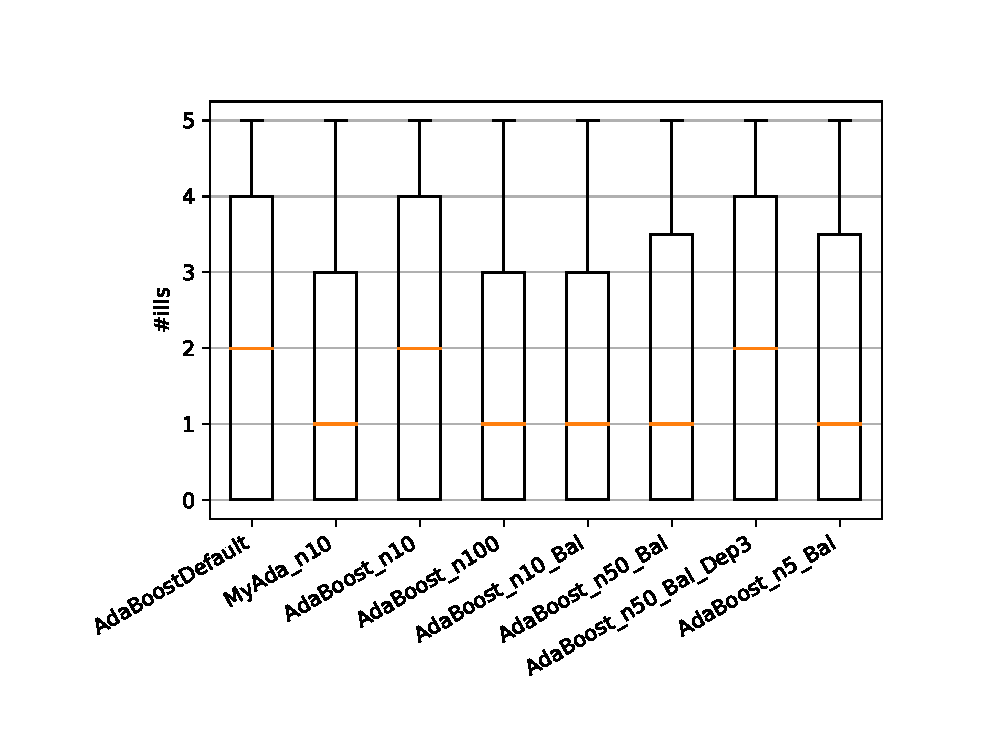
\includegraphics[scale = 0.80]{CC-AdaBoost-ills.eps}%
    \caption{Numero di ill-defined delle configurazioni di AdaBoost dell'ontologia CC}%
    \label{fig:ill1}% 
\end{figure}

\begin{figure}[hb]%
    \centering
    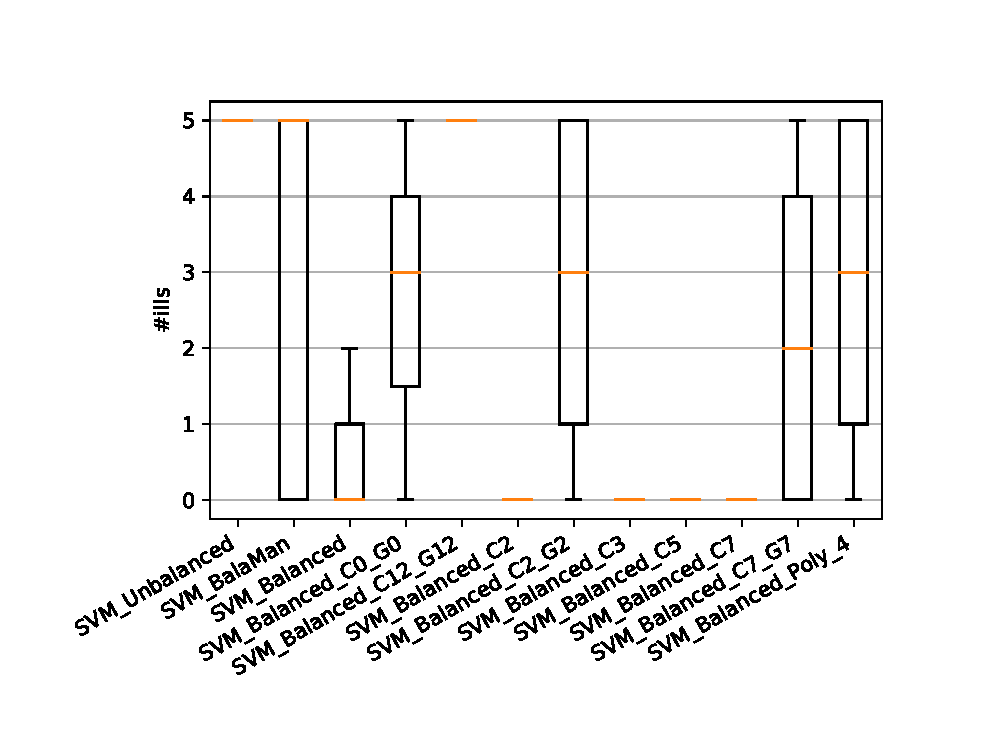
\includegraphics[scale = 0.80]{CC-SVM-ills.eps}%   
    \caption{Numero di ill-defined delle configurazioni di SVM dell'ontologia CC}%
    \label{figure:ill12}%
\end{figure}

\vspace*{\fill}

\topskip0pt
\vspace*{\fill}

\begin{figure}[ht]%
    \centering
    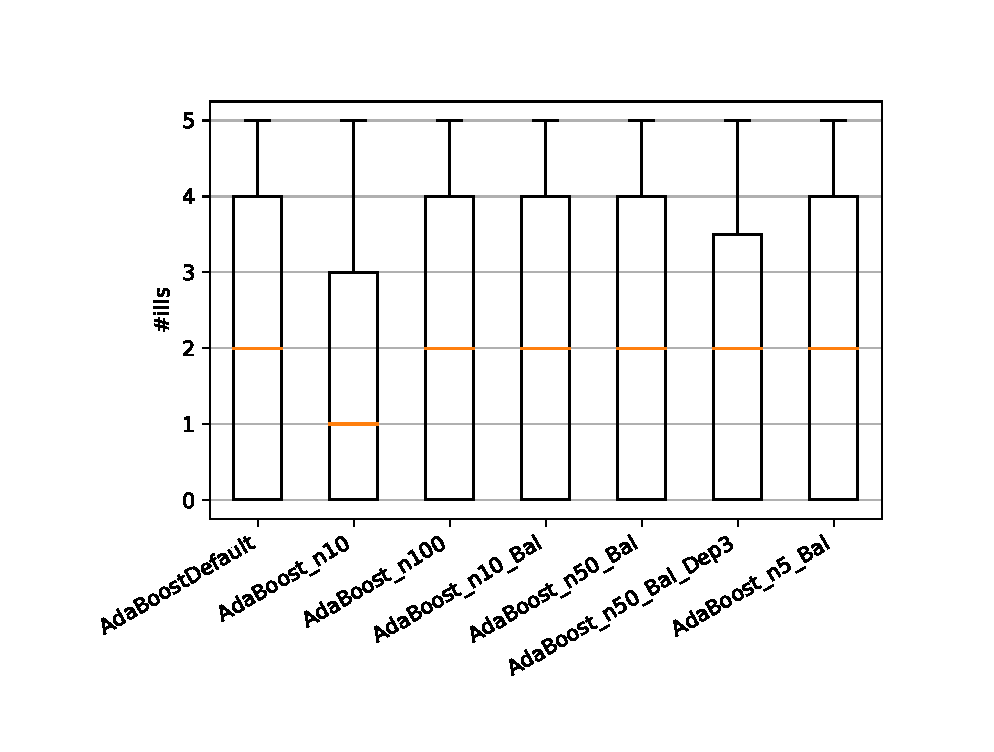
\includegraphics[scale = 0.80]{MF-AdaBoost-ills.eps}%
    \caption{Numero di ill-defined delle configurazioni di AdaBoost dell'ontologia MF}%
    \label{fig:ill13}% 
\end{figure}

\begin{figure}[hb]%
    \centering
    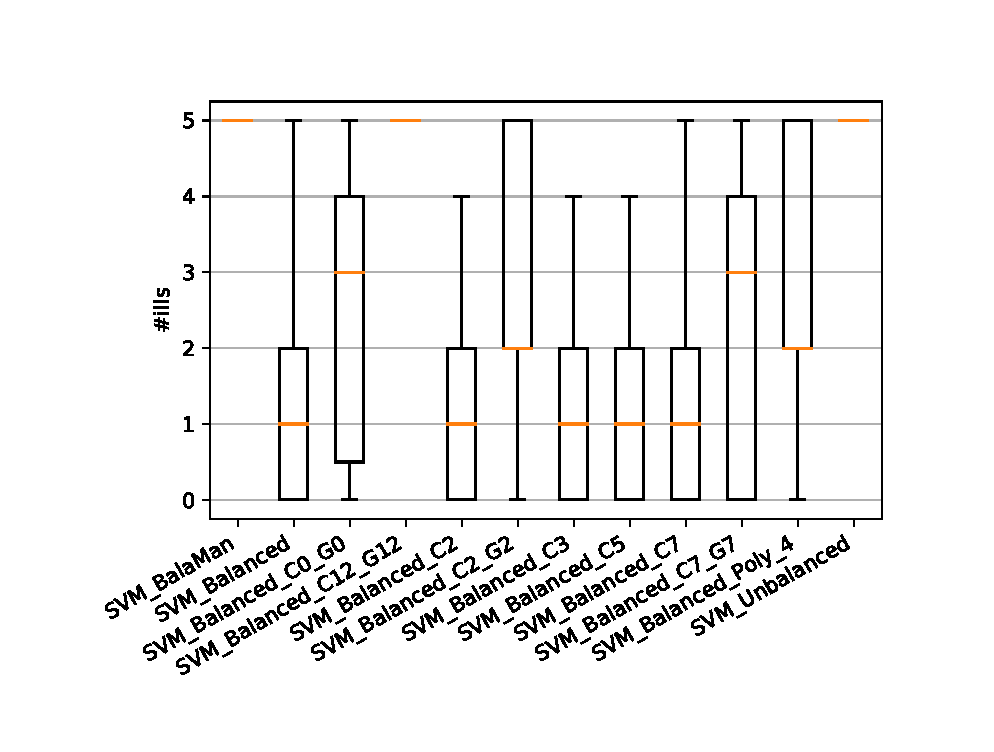
\includegraphics[scale = 0.80]{MF-SVM-ills.eps}%   
    \caption{Numero di ill-defined delle configurazioni di SVM dell'ontologia MF}%
    \label{figure:ill14}%
\end{figure}

\vspace*{\fill}

% //////////////////// LIVELLO 1 /////////////////

\topskip0pt
\vspace*{\fill}

\begin{figure}[hb]%
    \centering
    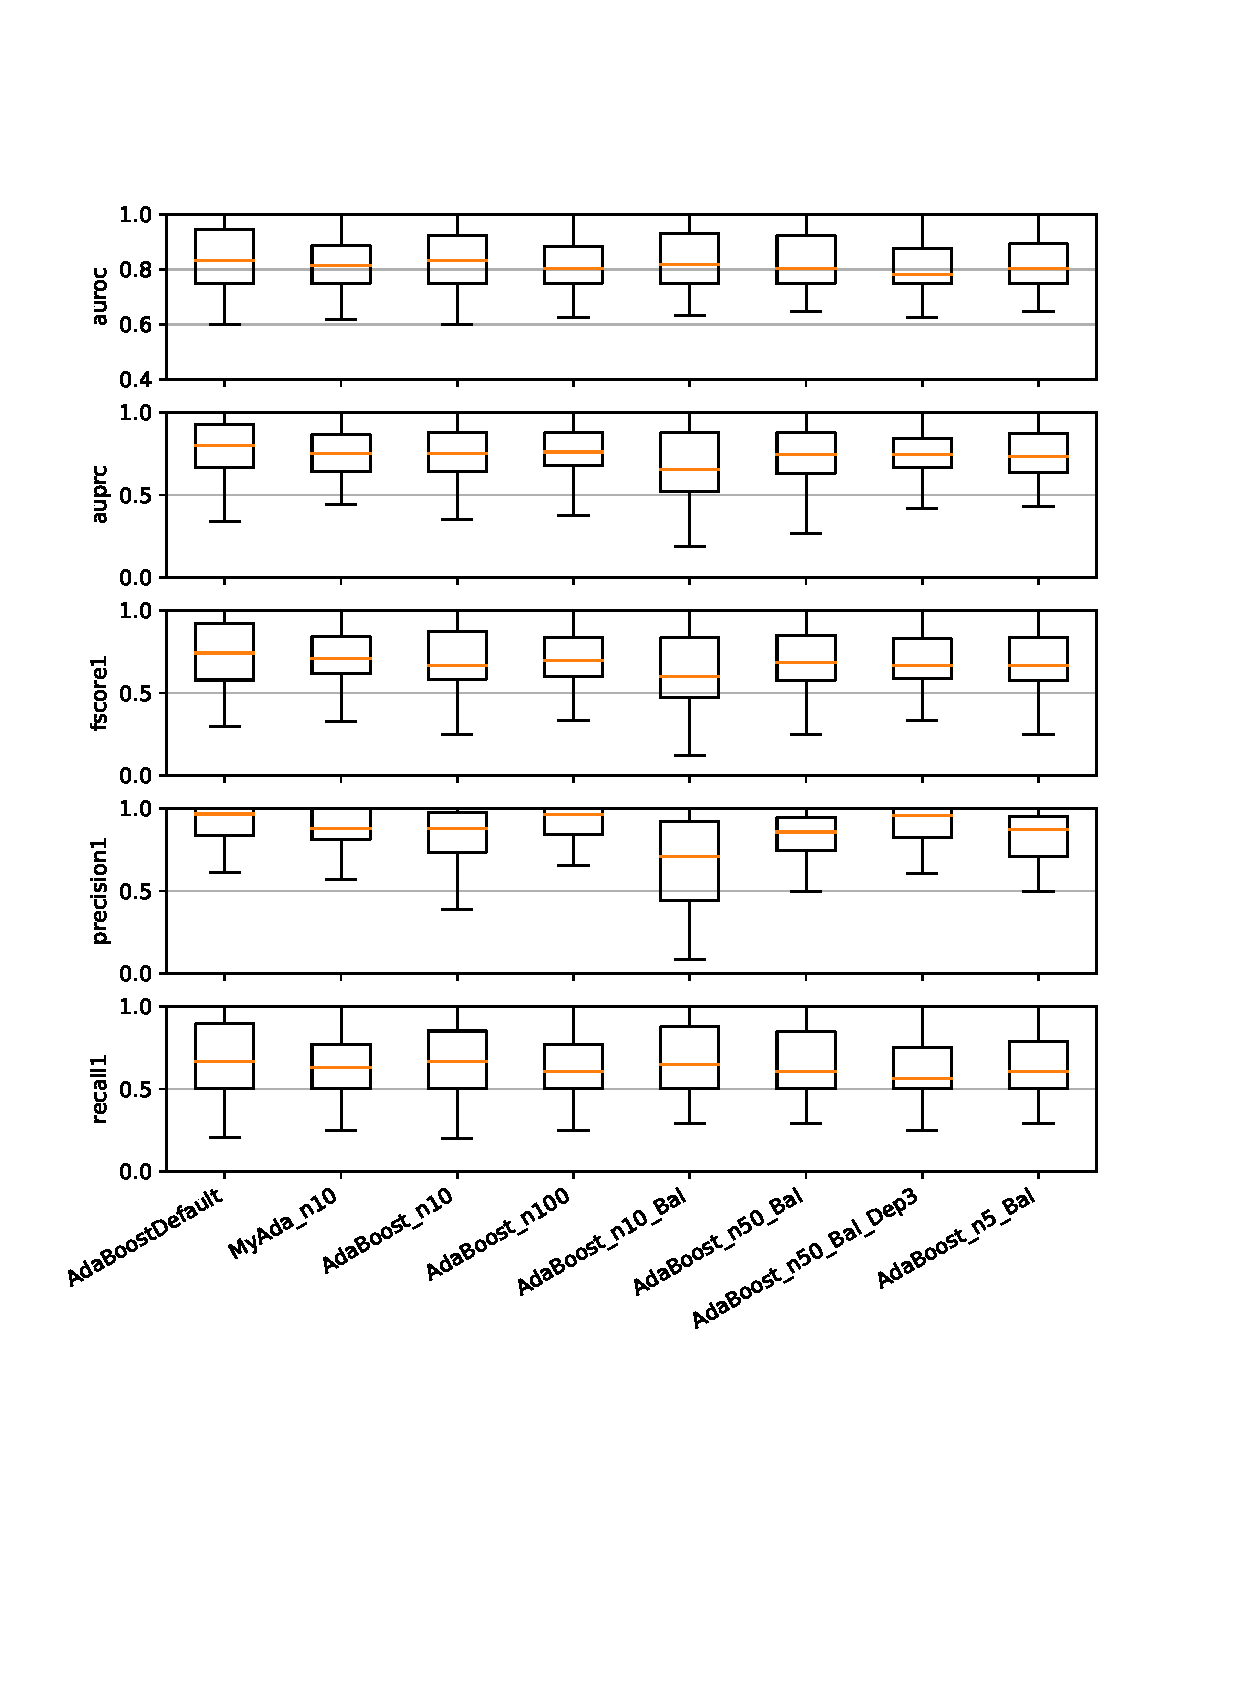
\includegraphics[scale = 0.80]{CC-AdaBoost-level1.eps}%   
    \caption{Confronto tra le metriche di diverse configurazioni di AdaBoost dell'ontologia CC}%
    \label{figure:liv1.1}%
\end{figure}

\vspace*{\fill}

\topskip0pt
\vspace*{\fill}

\begin{figure}[hb]%
    \centering
    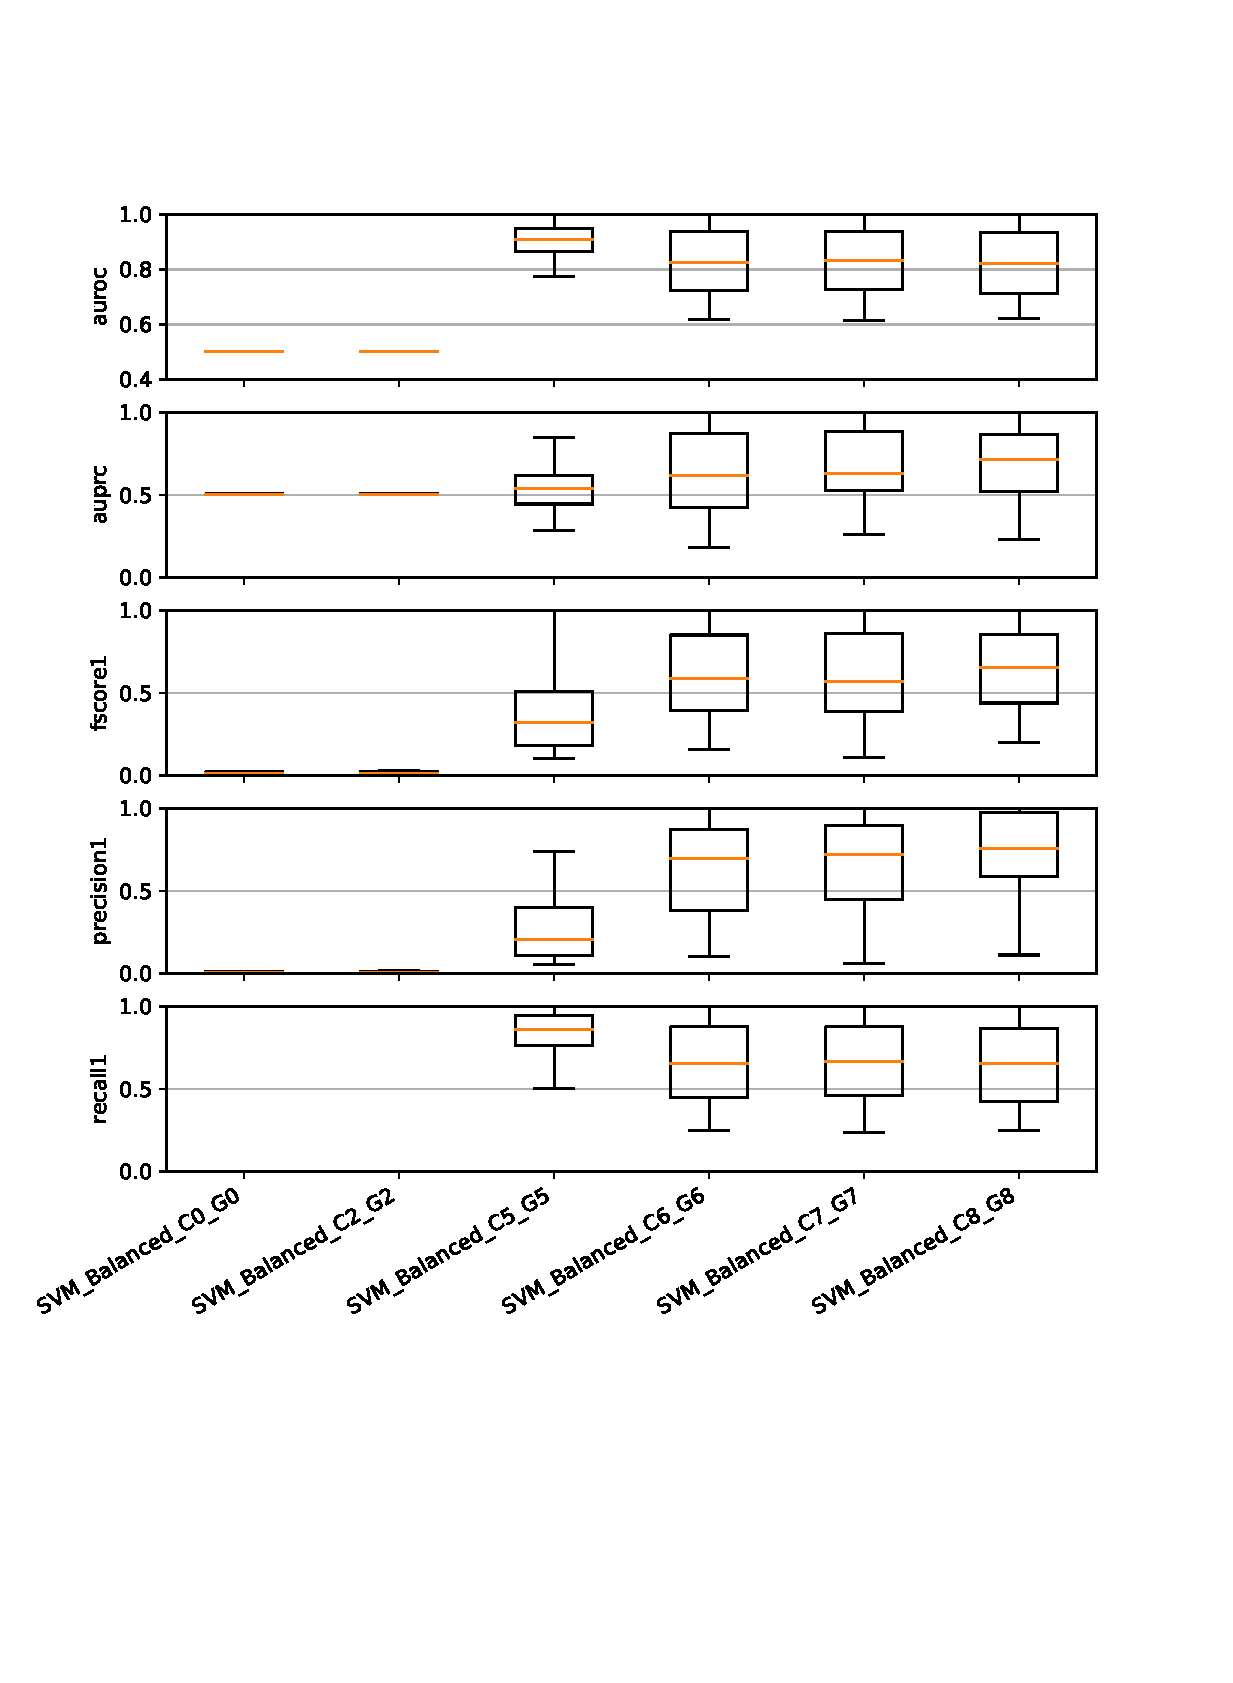
\includegraphics[scale = 0.80]{CC-SVM-level1.eps}%   
    \caption{Confronto tra le metriche di diverse configurazioni di SVM dell'ontologia CC}%
    \label{figure:liv1.2}%
\end{figure}

\vspace*{\fill}


\topskip0pt
\vspace*{\fill}

\begin{figure}[hb]%
    \centering
    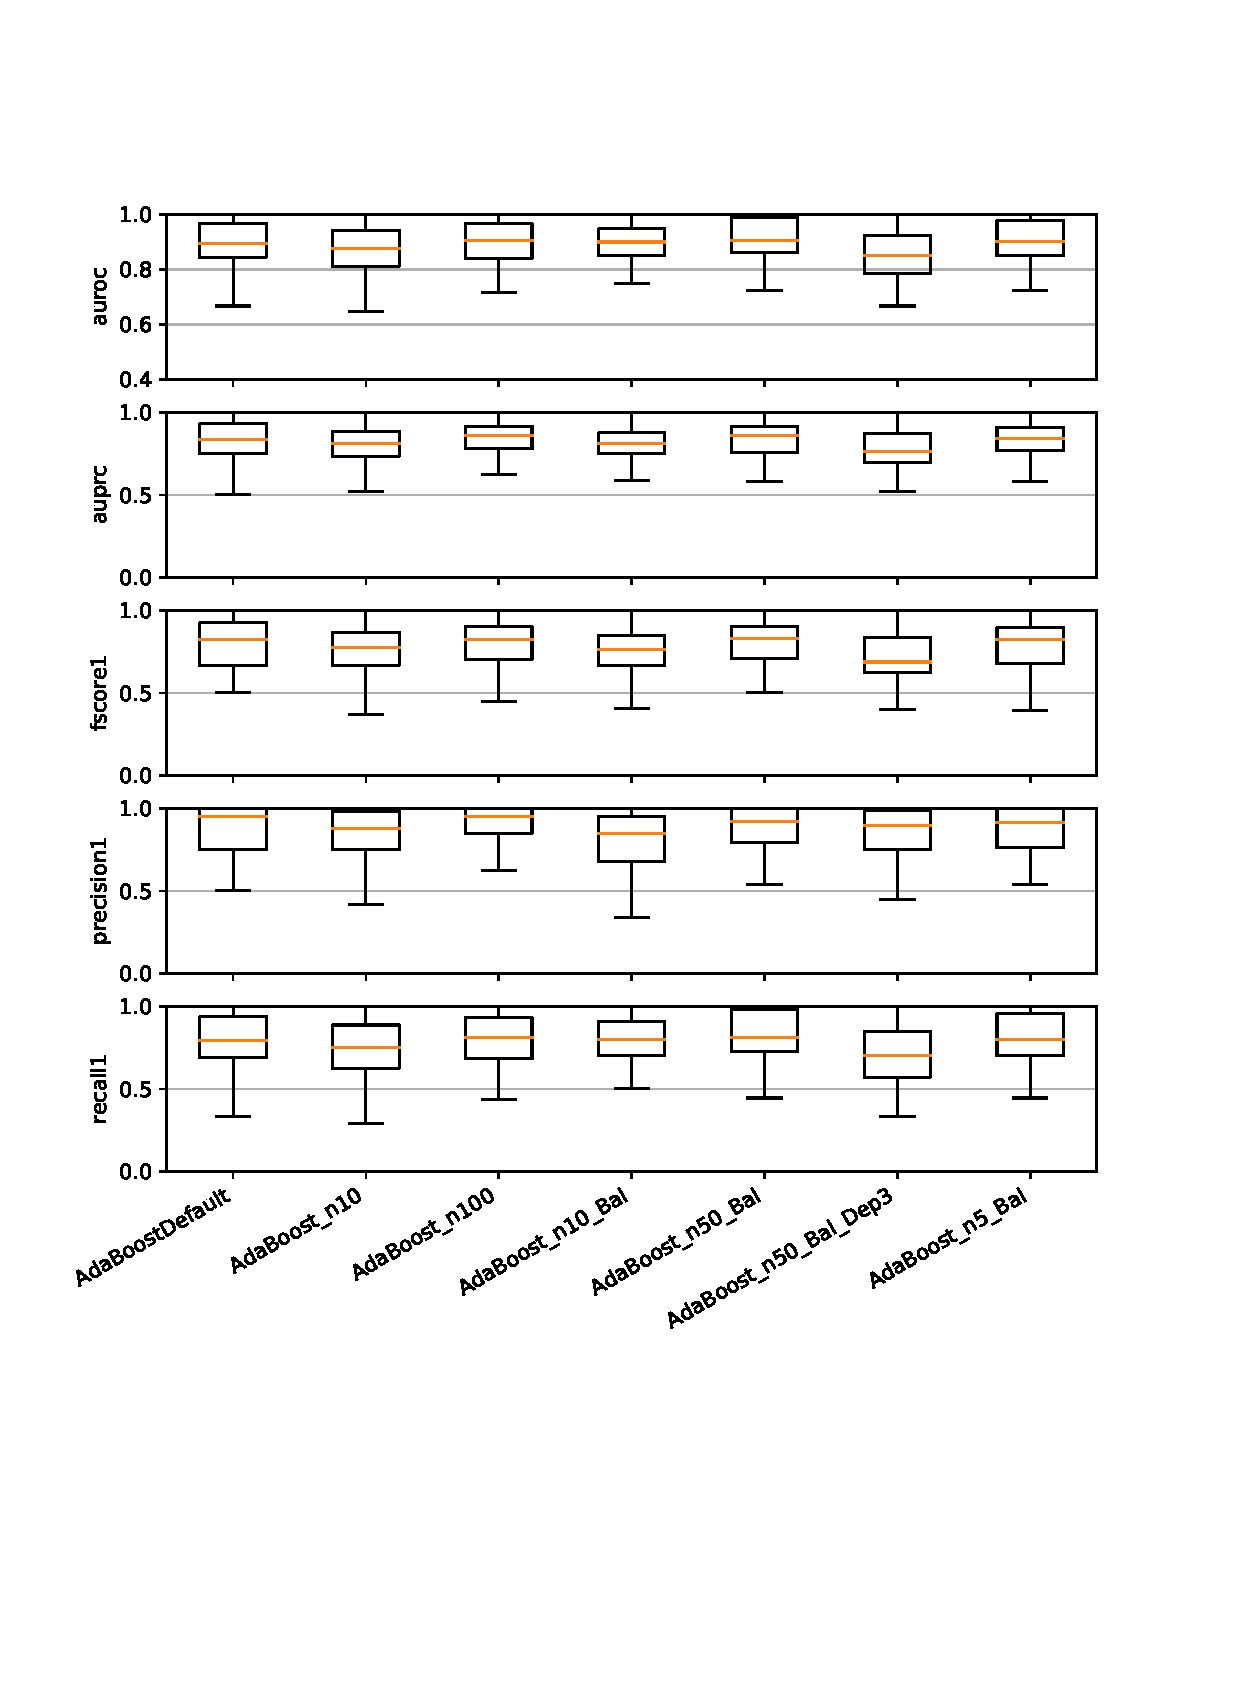
\includegraphics[scale = 0.80]{MF-AdaBoost-level1.eps}%   
    \caption{Confronto tra le metriche di diverse configurazioni di AdaBoost dell'ontologia MF}%
    \label{figure:liv1.3}%
\end{figure}

\vspace*{\fill}

\topskip0pt
\vspace*{\fill}

\begin{figure}[hb]%
    \centering
    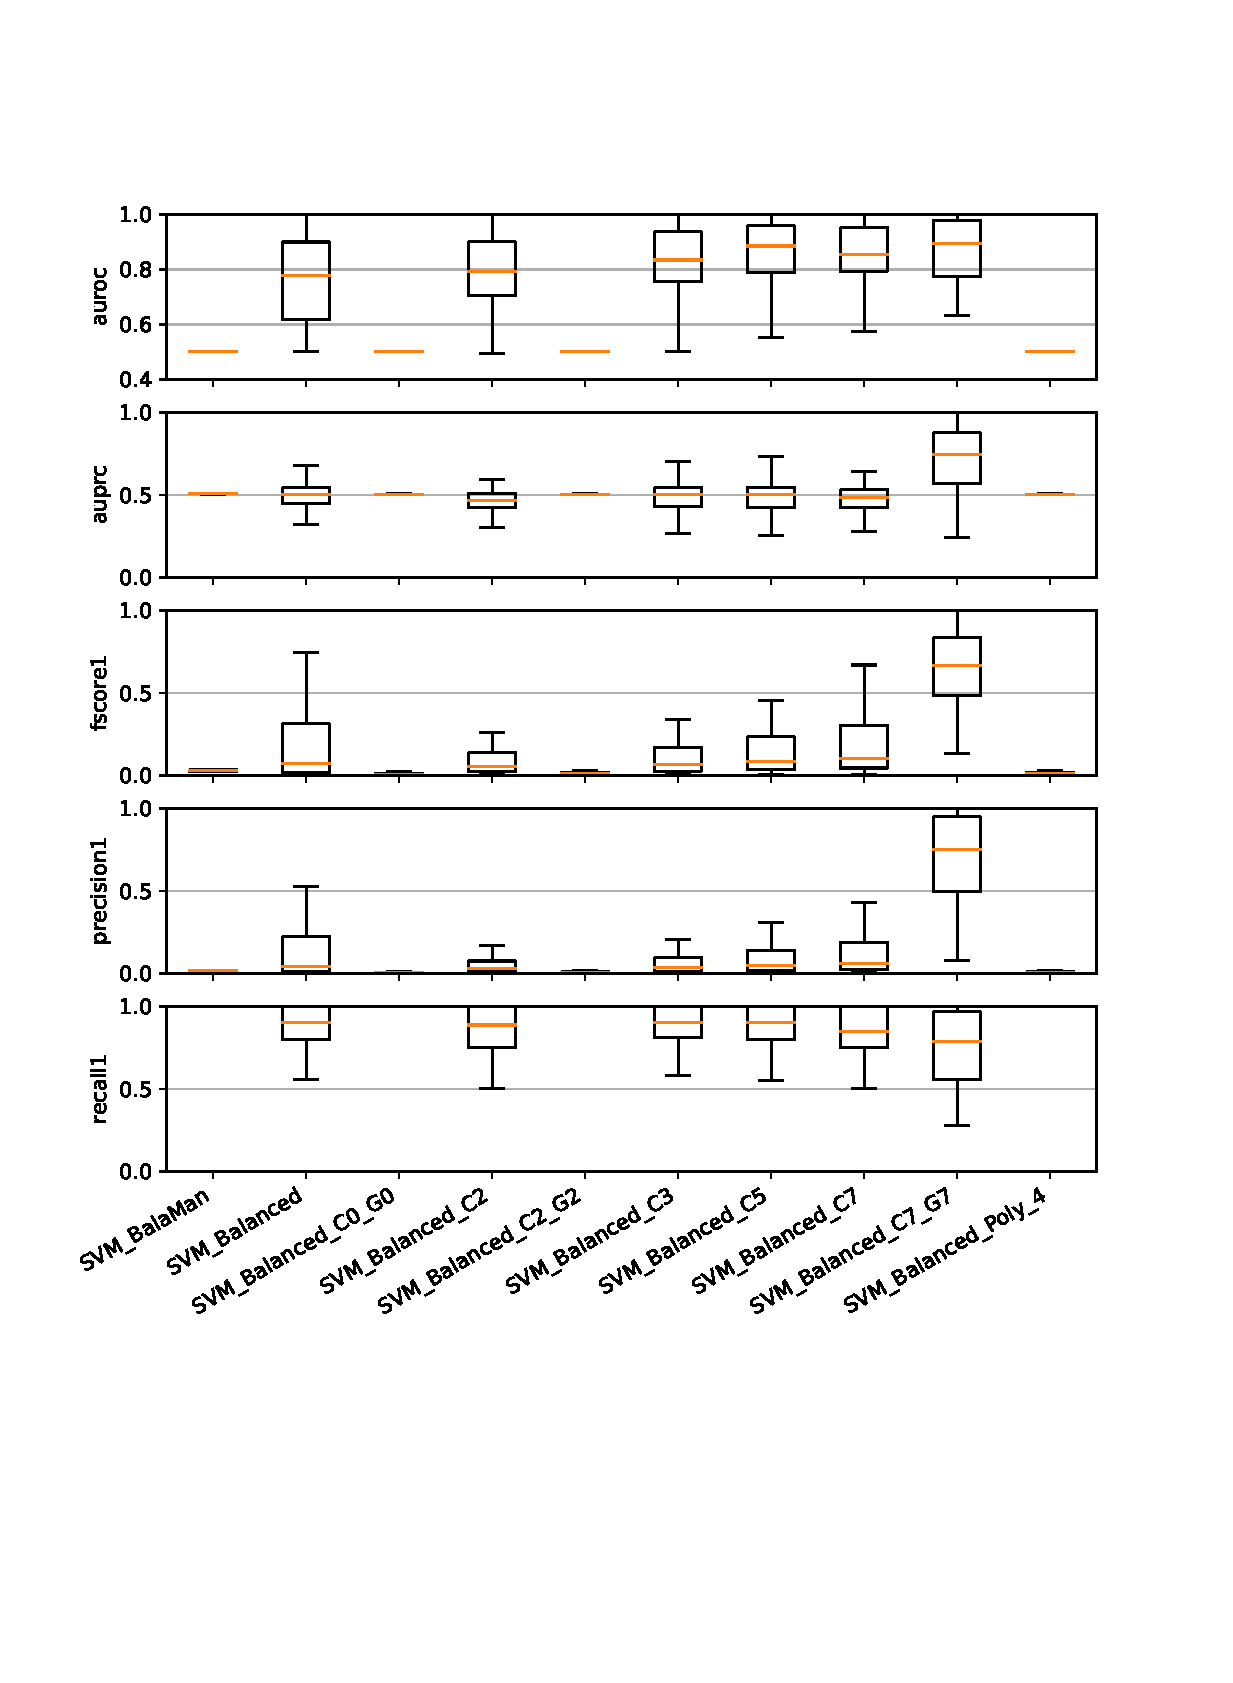
\includegraphics[scale = 0.80]{MF-SVM-level1.eps}%   
    \caption{Confronto tra le metriche di diverse configurazioni di SVM dell'ontologia MF}%
    \label{figure:liv1.4}%
\end{figure}

\vspace*{\fill}



% //////////////////// LIVELLO 2 /////////////////

\topskip0pt
\vspace*{\fill}

\begin{figure}[ht]%
    \centering
    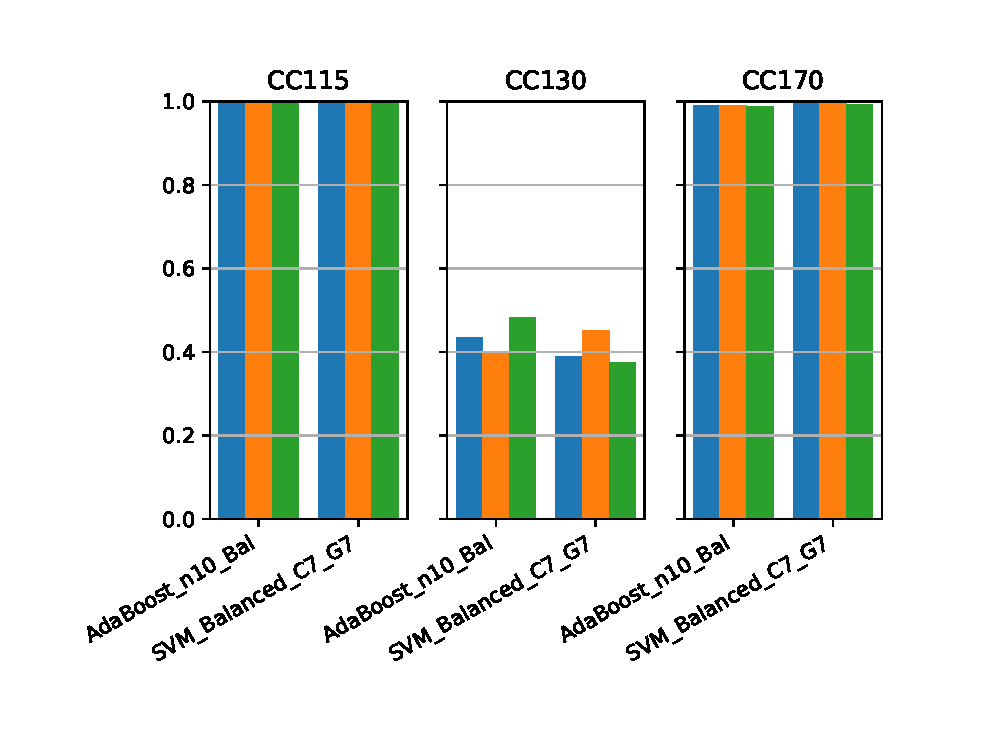
\includegraphics[scale = 0.80]{CC-level2.eps}%
    \caption{Confronto tra i classificatori che hanno le migliori performance su diverse classi dell'ontologia CC.}%
    \label{fig:liv2}% 
\end{figure}

\begin{figure}[hb]%
    \centering
    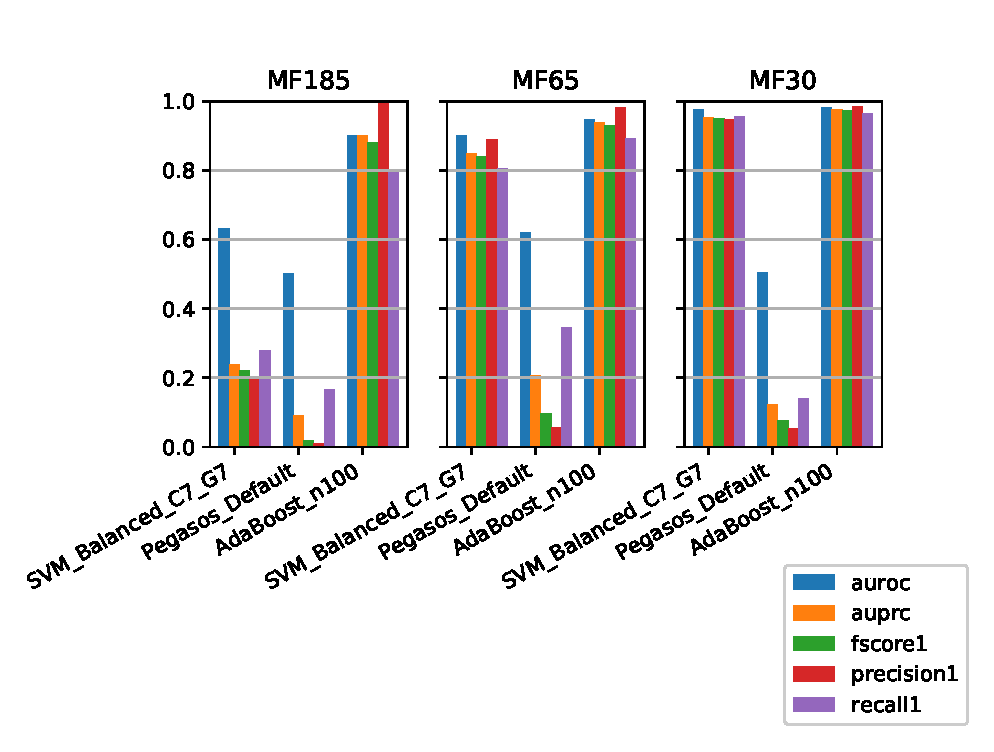
\includegraphics[scale = 0.80]{MF-level2.eps}%   
    \caption{Confronto tra i classificatori che hanno le migliori performance su diverse classi dell'ontologia MF.}%
    \label{figure:liv21}%
\end{figure}

\vspace*{\fill}


% //////////////////// LIVELLO 3 /////////////////

\topskip0pt
\vspace*{\fill}

\begin{figure}[ht]%
    \centering
    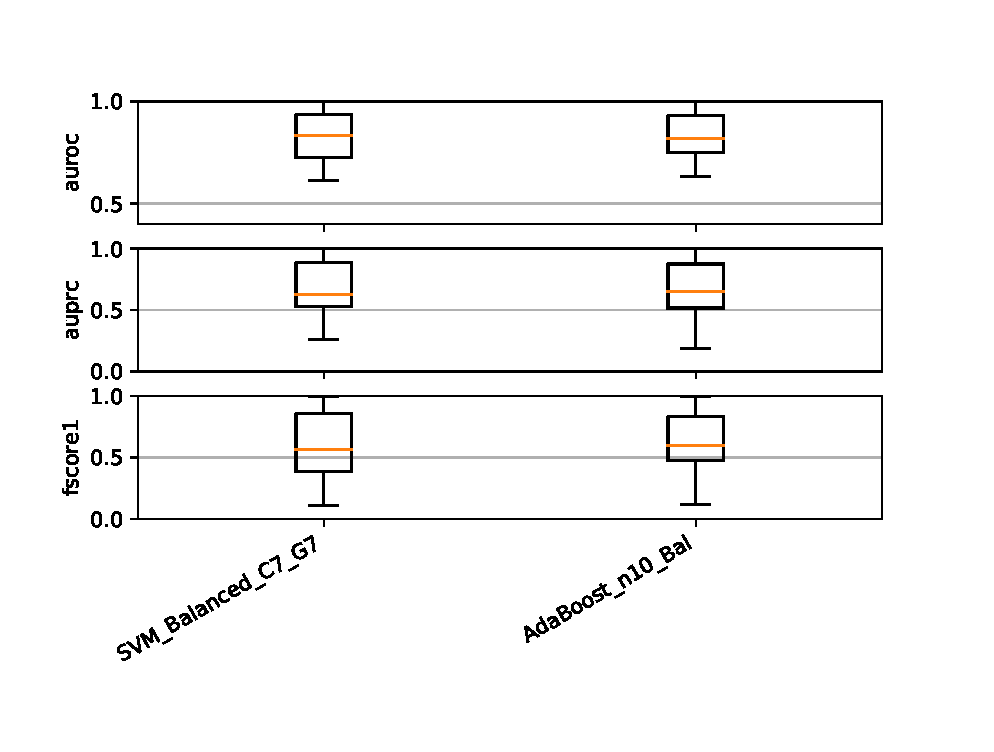
\includegraphics[scale = 0.80]{CC-level3.eps}%
    \caption{Confronto tra i migliori classificatori dell'ontologia CC}%
    \label{fig:liv3} 
\end{figure}

\begin{figure}[hb]%
    \centering
    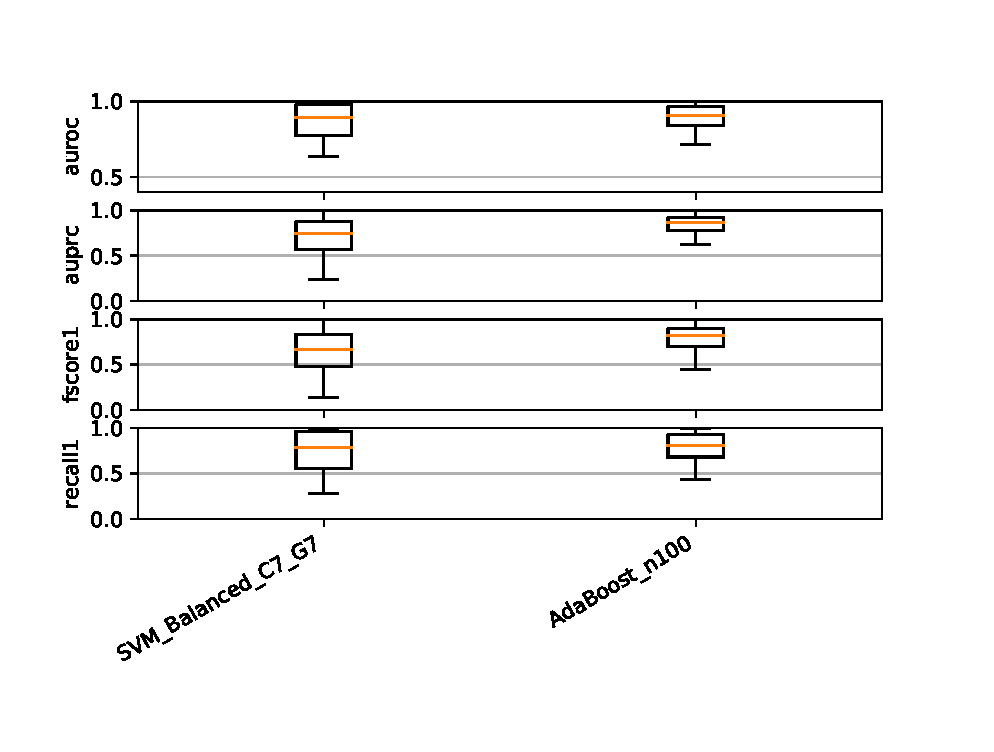
\includegraphics[scale = 0.80]{MF-level3.eps}%   
    \caption{Confronto tra i migliori classificatori dell'ontologia MF}%
    \label{figure:liv31}%
\end{figure}

\vspace*{\fill}

\appendix
\chapter{Software}
Il programma viene avviato eseguendo il file Python \textit{controller.py}. Questo file viene utilizzato per interfacciarsi con l'utente.
Di seguito viene mostrata la sintassi di esecuzione con i relativi parametri:

\begin{lstlisting}
python controller.py (ontologia) (configurazioni)
\end{lstlisting}
Il parametro \textbf{\textit{ontologia}} accetta come valori solo le stringhe \textit{CC} e \textit{MF}. \\
Il parametro \textbf{\textit{configurazioni}} accetta come valori i nomi delle configurazioni della Tabella~\ref{tab:b1} e della Tabella~\ref{tab:b2} separati da virgole. Se durante l'inserimento si verifica un errore di sintassi o non viene inserito nessun parametro, vengono eseguite tutte le configurazioni disponibili.

Il listato del codice implementato è descritto nelle pagine seguenti.

\newpage

% Viene impostato lo stile del codice relativo a Python
\lstset{style=customp}

\lstinputlisting{controller.py}

\newpage

\lstinputlisting{dataload.py}

\newpage

\lstinputlisting{metrics.py}

\end{document}